\documentclass[oneside]{book}

\usepackage{amsmath, amsthm, amssymb, amsfonts}
\usepackage{thmtools}
\usepackage{graphicx}
\usepackage{setspace}
\usepackage{geometry}
\usepackage{float}
\usepackage{hyperref}
\usepackage[utf8]{inputenc}
\usepackage[english]{babel}
\usepackage{framed}
\usepackage[dvipsnames]{xcolor}
\usepackage{environ}
\usepackage{tcolorbox}
\tcbuselibrary{theorems, skins, breakable}

\setstretch{1.2}
\geometry{
    textheight=9in,
    textwidth=5.5in,
    top=1in,
    headheight=12pt,
    headsep=25pt,
    footskip=30pt
}

% Variables
\def\notetitle{MATH 165\\Linear Algebra \& Diff. Equation\\Final \\Notes with Examples}
\def\noteauthor{
    \textbf{Professor Kalyani Madhu} \\ 
    % {\LaTeX} 
    by Ethan\\
    University of Rochester}
\def\notedate{Spring 2024}

% The theorem system and user-defined commands
% Theorem System
% The following boxes are provided:
%   Definition:     \defn 
%   Theorem:        \thm 
%   Lemma:          \lem
%   Corollary:      \cor
%   Proposition:    \prop   
%   Claim:          \clm
%   Fact:           \fact
%   Proof:          \pf
%   Example:        \ex
%   Remark:         \rmk (sentence), \rmkb (block)
% Suffix
%   r:              Allow Theorem/Definition to be referenced, e.g. thmr
%   p:              Add a short proof block for Lemma, Corollary, Proposition or Claim, e.g. lemp
%                   For theorems, use \pf for proof blocks

% Definition
\newtcbtheorem[number within=section]{mydefinition}{Definition}
{
    enhanced,
    frame hidden,
    titlerule=0mm,
    toptitle=1mm,
    bottomtitle=1mm,
    fonttitle=\bfseries\large,
    coltitle=black,
    colbacktitle=green!20!white,
    colback=green!10!white,
}{defn}

\NewDocumentCommand{\defn}{m+m}{
    \begin{mydefinition}{#1}{}
        #2
    \end{mydefinition}
}

\NewDocumentCommand{\defnr}{mm+m}{
    \begin{mydefinition}{#1}{#2}
        #3
    \end{mydefinition}
}

% Theorem
\newtcbtheorem[use counter from=mydefinition]{mytheorem}{Theorem}
{
    enhanced,
    frame hidden,
    titlerule=0mm,
    toptitle=1mm,
    bottomtitle=1mm,
    fonttitle=\bfseries\large,
    coltitle=black,
    colbacktitle=cyan!20!white,
    colback=cyan!10!white,
}{thm}

\NewDocumentCommand{\thm}{m+m}{
    \begin{mytheorem}{#1}{}
        #2
    \end{mytheorem}
}

\NewDocumentCommand{\thmr}{mm+m}{
    \begin{mytheorem}{#1}{#2}
        #3
    \end{mytheorem}
}

% Lemma
\newtcbtheorem[use counter from=mydefinition]{mylemma}{Lemma}
{
    enhanced,
    frame hidden,
    titlerule=0mm,
    toptitle=1mm,
    bottomtitle=1mm,
    fonttitle=\bfseries\large,
    coltitle=black,
    colbacktitle=violet!20!white,
    colback=violet!10!white,
}{lem}

\NewDocumentCommand{\lem}{m+m}{
    \begin{mylemma}{#1}{}
        #2
    \end{mylemma}
}

\newenvironment{lempf}{
	{\noindent{\it \textbf{Proof for Lemma}}}
	\tcolorbox[blanker,breakable,left=5mm,parbox=false,
    before upper={\parindent15pt},
    after skip=10pt,
	borderline west={1mm}{0pt}{violet!20!white}]
}{
    \textcolor{violet!20!white}{\hbox{}\nobreak\hfill$\blacksquare$} 
    \endtcolorbox
}

\NewDocumentCommand{\lemp}{m+m+m}{
    \begin{mylemma}{#1}{}
        #2
    \end{mylemma}

    \begin{lempf}
        #3
    \end{lempf}
}

% Corollary
\newtcbtheorem[use counter from=mydefinition]{mycorollary}{Corollary}
{
    enhanced,
    frame hidden,
    titlerule=0mm,
    toptitle=1mm,
    bottomtitle=1mm,
    fonttitle=\bfseries\large,
    coltitle=black,
    colbacktitle=orange!20!white,
    colback=orange!10!white,
}{cor}

\NewDocumentCommand{\cor}{+m}{
    \begin{mycorollary}{}{}
        #1
    \end{mycorollary}
}

\newenvironment{corpf}{
	{\noindent{\it \textbf{Proof for Corollary.}}}
	\tcolorbox[blanker,breakable,left=5mm,parbox=false,
    before upper={\parindent15pt},
    after skip=10pt,
	borderline west={1mm}{0pt}{orange!20!white}]
}{
    \textcolor{orange!20!white}{\hbox{}\nobreak\hfill$\blacksquare$} 
    \endtcolorbox
}

\NewDocumentCommand{\corp}{m+m+m}{
    \begin{mycorollary}{}{}
        #1
    \end{mycorollary}

    \begin{corpf}
        #2
    \end{corpf}
}

% Proposition
\newtcbtheorem[use counter from=mydefinition]{myproposition}{Proposition}
{
    enhanced,
    frame hidden,
    titlerule=0mm,
    toptitle=1mm,
    bottomtitle=1mm,
    fonttitle=\bfseries\large,
    coltitle=black,
    colbacktitle=yellow!30!white,
    colback=yellow!20!white,
}{prop}

\NewDocumentCommand{\prop}{+m}{
    \begin{myproposition}{}{}
        #1
    \end{myproposition}
}

\newenvironment{proppf}{
	{\noindent{\it \textbf{Proof for Proposition.}}}
	\tcolorbox[blanker,breakable,left=5mm,parbox=false,
    before upper={\parindent15pt},
    after skip=10pt,
	borderline west={1mm}{0pt}{yellow!30!white}]
}{
    \textcolor{yellow!30!white}{\hbox{}\nobreak\hfill$\blacksquare$} 
    \endtcolorbox
}

\NewDocumentCommand{\propp}{+m+m}{
    \begin{myproposition}{}{}
        #1
    \end{myproposition}

    \begin{proppf}
        #2
    \end{proppf}
}

% Claim
\newtcbtheorem[use counter from=mydefinition]{myclaim}{Claim}
{
    enhanced,
    frame hidden,
    titlerule=0mm,
    toptitle=1mm,
    bottomtitle=1mm,
    fonttitle=\bfseries\large,
    coltitle=black,
    colbacktitle=pink!30!white,
    colback=pink!20!white,
}{clm}


\NewDocumentCommand{\clm}{m+m}{
    \begin{myclaim*}{#1}{}
        #2
    \end{myclaim*}
}

\newenvironment{clmpf}{
	{\noindent{\it \textbf{Proof for Claim.}}}
	\tcolorbox[blanker,breakable,left=5mm,parbox=false,
    before upper={\parindent15pt},
    after skip=10pt,
	borderline west={1mm}{0pt}{pink!30!white}]
}{
    \textcolor{pink!30!white}{\hbox{}\nobreak\hfill$\blacksquare$} 
    \endtcolorbox
}

\NewDocumentCommand{\clmp}{m+m+m}{
    \begin{myclaim*}{#1}{}
        #2
    \end{myclaim*}

    \begin{clmpf}
        #3
    \end{clmpf}
}

% Fact
\newtcbtheorem[use counter from=mydefinition]{myfact}{Fact}
{
    enhanced,
    frame hidden,
    titlerule=0mm,
    toptitle=1mm,
    bottomtitle=1mm,
    fonttitle=\bfseries\large,
    coltitle=black,
    colbacktitle=purple!20!white,
    colback=purple!10!white,
}{fact}

\NewDocumentCommand{\fact}{+m}{
    \begin{myfact}{}{}
        #1
    \end{myfact}
}


% Proof
\NewDocumentCommand{\pf}{+m}{
    \begin{proof}
        [\noindent\textbf{Proof.}]
        #1
    \end{proof}
}

% Example
\newenvironment{example}{%
    \par
    \vspace{5pt}
	\begin{minipage}{\textwidth}
		\noindent\textbf{Example.}
		\tcolorbox[blanker,breakable,left=5mm,parbox=false,
	    before upper={\parindent15pt},
	    after skip=10pt,
		borderline west={1mm}{0pt}{cyan!10!white}]
}{%
		\endtcolorbox
	\end{minipage}
    \vspace{5pt}
}

\NewDocumentCommand{\ex}{+m}{
    \begin{example}
        #1
    \end{example}
}


% Remark
\NewDocumentCommand{\rmk}{+m}{
    {\it \color{blue!50!white}#1}
}

\newenvironment{remark}{
    \par
    \vspace{5pt}
    \begin{minipage}{\textwidth}
        {\par\noindent{\textbf{Remark.}}}
        \tcolorbox[blanker,breakable,left=5mm,
        before skip=10pt,after skip=10pt,
        borderline west={1mm}{0pt}{cyan!10!white}]
}{
        \endtcolorbox
    \end{minipage}
    \vspace{5pt}
}

\NewDocumentCommand{\rmkb}{+m}{
    \begin{remark}
        #1
    \end{remark}
}


\newcommand{\lcm}{\operatorname{lcm}}




% ------------------------------------------------------------------------------

\begin{document}
\title{\textbf{
    \LARGE{\notetitle} \vspace*{10\baselineskip}}
    }
\author{\noteauthor}
\date{\notedate}

\maketitle
\newpage

\tableofcontents
\newpage

% ------------------------------------------------------------------------------
\chapter{Linear Transformations}
\section{Lecture 17 \& 18: Linear Transformation, Kernel \& Range}
\rmk{
    This lecture covers: 
    \begin{itemize}
        \item 6.1 Definition of Linear Transformations
        \item 6.2 Transformations of $\mathbb{R}^2$
        \item 6.3 The Kernel and Range of a Linear Transformation
    \end{itemize}
}

\subsection{Definition of Linear Transformations}
\subsubsection{Definition}
\defn{Mapping}{
    Let $V$ and $W$ be vector spaces. A \textbf{mapping} $T$ from $V$ to $W$ is a rule that assigns to each vector $\vec{v}$ in $V$ precisely one vector $\vec{w} = T(\vec{v})$. We write $T: V \to W$.
}

Linear Transformation is a kind of mapping that preserves the operations of vector addition and scalar multiplication.

\defn{Linear Transformation}{
    Let $V$ and $W$ be vector spaces over the same field. A mapping $T: V \to W$ is a \textbf{linear transformation} if for all $\vec{v}_1, \vec{v}_2 \in V$ and all scalars $c$:
    \begin{enumerate}
        \item $T(\vec{u} + \vec{v}) = T(\vec{u}) + T(\vec{v})$ for all $\vec{u}, \vec{v} \in V$
        \item $T(c\vec{v}) = cT(\vec{v})$ for all $\vec{v} \in V$
    \end{enumerate}
    In the above equations, the operations on the left of the equal signs are the ones defined in the domain $V$ and
the ones on the right of the equal signs are the ones defined in the codomain $W$.
}

\begin{figure}
    \center
    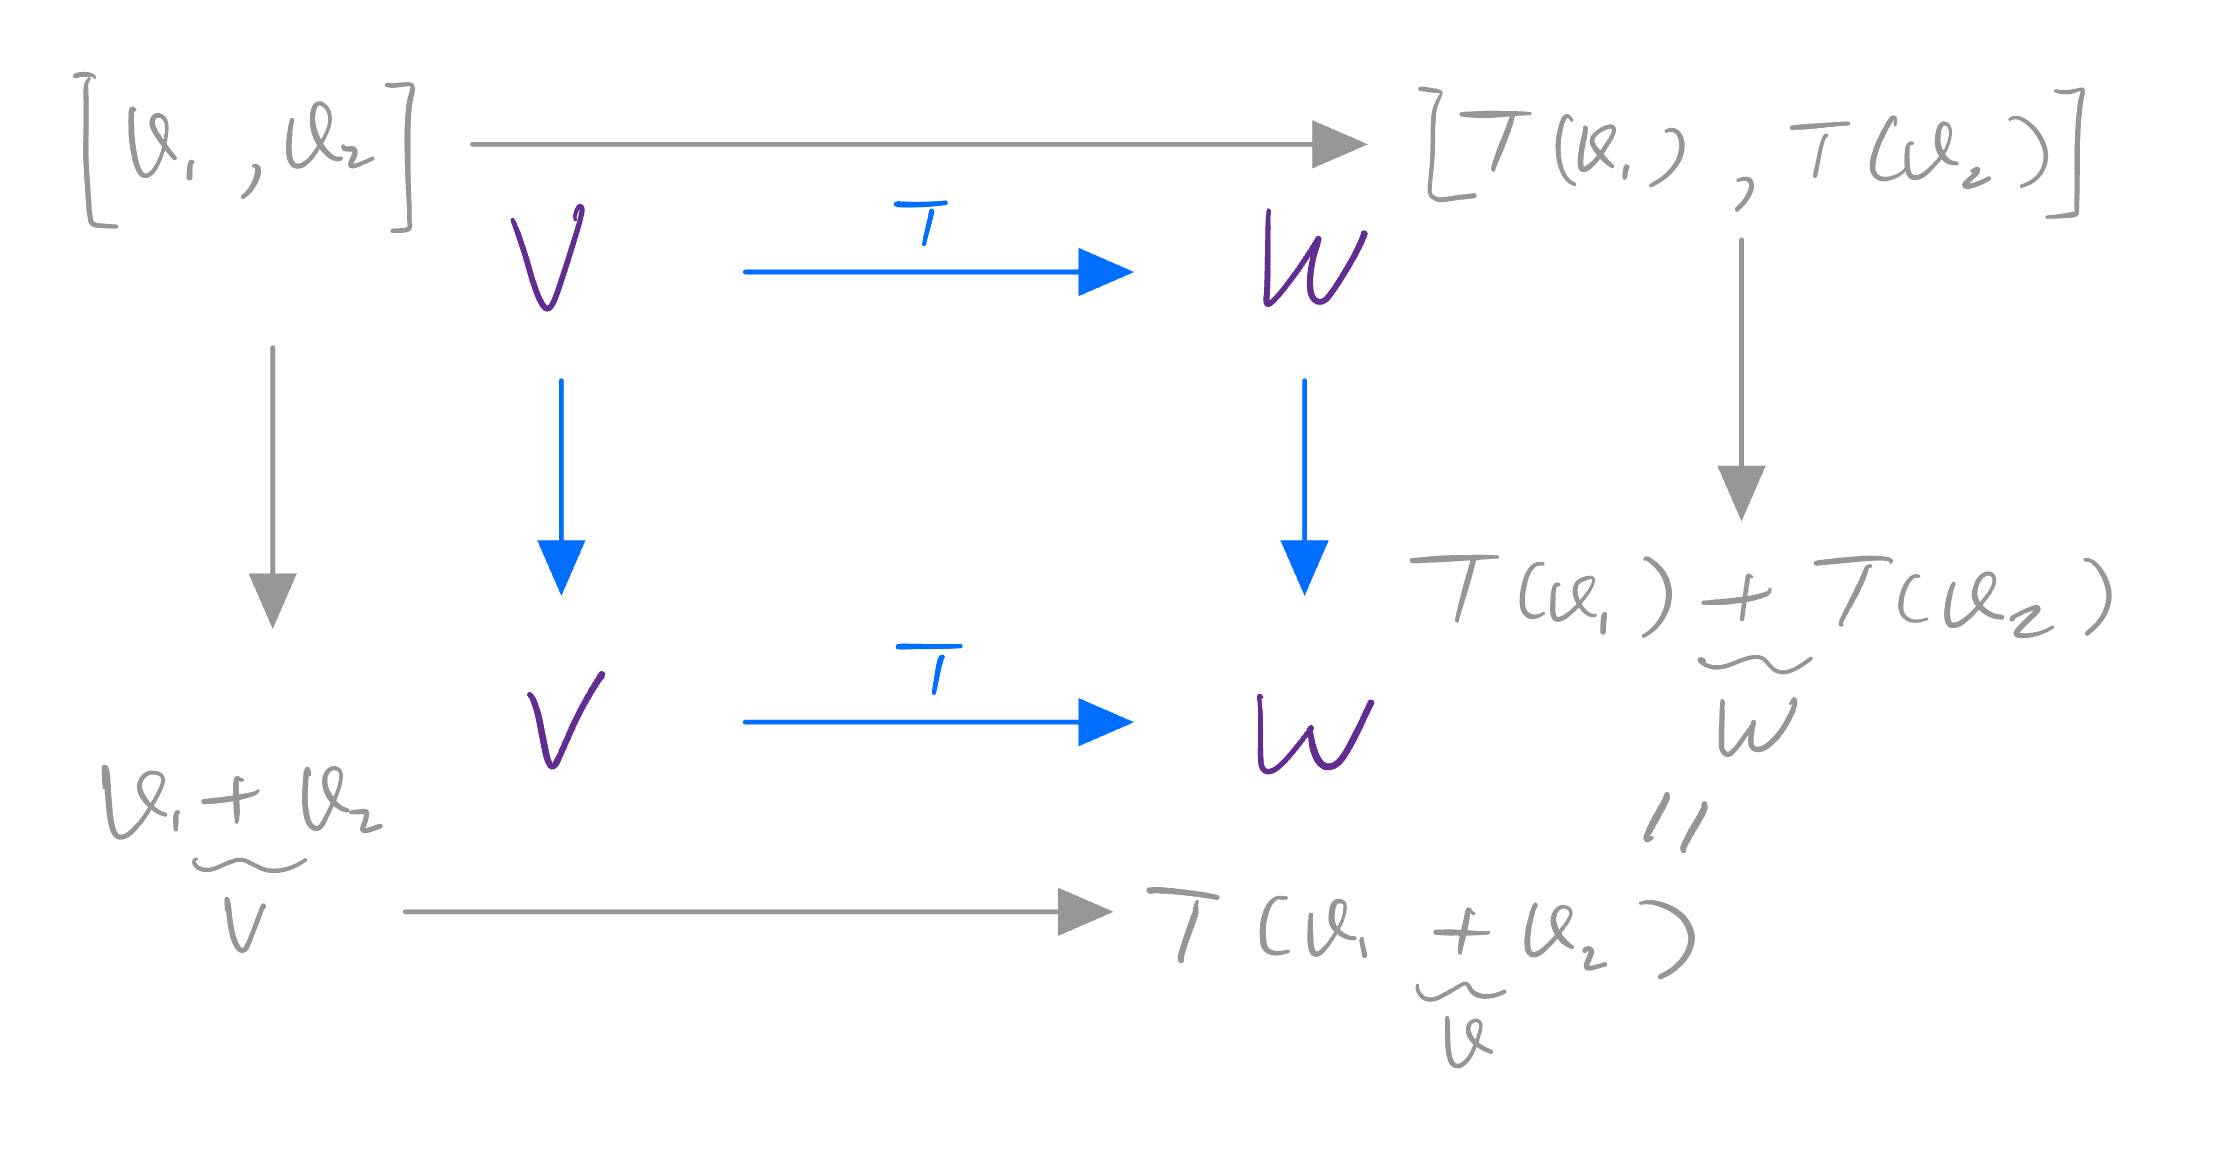
\includegraphics[width=0.5\textwidth]{img/Note 25 Mar 2024.jpeg}
    \caption{Linear Transformation Diagram}
\end{figure}
\subsection{How to prove a transformation is linear}

\ex{
    Show $T:P_2 \to P_4$ given by $T(p) = x^2 p(x)$ is linear. 
    \begin{proof}
        We need to show that $T(p + q) = T(p) + T(q)$ and $T(cp) = cT(p)$ for all $p, q \in P_2$ and $c \in \mathbb{R}$. \\
        Let $p, q \in P_2$ and $c \in \mathbb{R}$. \\
        \[
            T(p + q) = x^2(p + q)(x) = x^2p(x) + x^2q(x) = T(p) + T(q)
        \]
        \[T(cp) = x^2(cp)(x) = cx^2p(x) = cT(p)\]
        Thus, $T$ is linear.

    \end{proof}

}

Here's a short-cut to test if a transformation is linear:

\thmr{}{}{
    Let $V, W$ be vector spaces over field $F$. A mapping $T: V \to W$ is a linear transformation if and only if for all $\lambda_1, \lambda_2 \in F$ and all $\vec{v}_1, \vec{v}_2 \in V$:
    \[
        T(\lambda_1\vec{v}_1 + \lambda_2\vec{v}_2) = \lambda_1T(\vec{v}_1) + \lambda_2T(\vec{v}_2)
    \]
}



\ex{
    Which of the following are linear transformations?
\begin{enumerate}
    \item $T: P_2 \to P_1$ given by $T(p) = p'$
    \item $T: \mathbb{R} \to \mathbb{R}^2$ given by $T(x) = (x, 2x)$
    \item $T: \mathbb{R} \to \mathbb{R}^2$ given by $T(x) = (x, x^2)$
\end{enumerate}
\begin{proof} We can use the definition of linear transformations to check each case: 
    \begin{enumerate}
        \item $T(p) = p'$ is linear since $T(\lambda_1p_1 + \lambda_2p_2) = (\lambda_1p_1 + \lambda_2p_2)' = \lambda_1p_1' + \lambda_2p_2' = \lambda_1T(p_1) + \lambda_2T(p_2)$
        \item $T(x) = (x, 2x)$ is linear since $T(\lambda_1x_1 + \lambda_2x_2) = (\lambda_1x_1 + \lambda_2x_2, 2(\lambda_1x_1 + \lambda_2x_2)) = \lambda_1(x_1, 2x_1) + \lambda_2(x_2, 2x_2) = \lambda_1T(x_1) + \lambda_2T(x_2)$
        \item $T(x) = (x, x^2)$ is not linear since $T(\lambda_1x_1 + \lambda_2x_2) = (\lambda_1x_1 + \lambda_2x_2, (\lambda_1x_1 + \lambda_2x_2)^2) \neq \lambda_1(x_1, x_1^2) + \lambda_2(x_2, x_2^2) = \lambda_1T(x_1) + \lambda_2T(x_2)$
    \end{enumerate}
\end{proof}
}


\ex{
    $T: \mathbb{R}^2 \to P_1(\mathbb{R})$ given by $T(a, b) = a + bx$ is linear.
    \begin{proof}
        We want to show: $T(\lambda_1(a_1, b_1) + \lambda_2(a_2, b_2)) = \lambda_1T(a_1, b_1) + \lambda_2T(a_2, b_2)$
        \[
            T(\lambda_1(a_1, b_1) + \lambda_2(a_2, b_2)) = T(\lambda_1a_1 + \lambda_2a_2, \lambda_1b_1 + \lambda_2b_2) = (\lambda_1a_1 + \lambda_2a_2) + (\lambda_1b_1 + \lambda_2b_2)x
        \]
        \[
            \lambda_1T(a_1, b_1) + \lambda_2T(a_2, b_2) = \lambda_1(a_1 + b_1x) + \lambda_2(a_2 + b_2x) = (\lambda_1a_1 + \lambda_2a_2) + (\lambda_1b_1 + \lambda_2b_2)x
        \] \\
        Therefore, $T(\lambda_1(a_1, b_1) + \lambda_2(a_2, b_2)) = \lambda_1T(a_1, b_1) + \lambda_2T(a_2, b_2)$ \\
        Thus, $T$ is linear.
    
    \end{proof}
        
}

\subsubsection{Three very important examples of linear transformations}
\ex{
    \textbf{1:} A transformation given by a matrix: $T : \mathbb{R}^n \to \mathbb{R}^m$ given by $T(x) = Ax$ where $A$ is a fixed $m \times n$ matrix. \\
    \rmkb{Note that the domain of $T$ is $\mathbb{R}^n$ and the codomain is $\mathbb{R}^m$ – we reverse the order in which the dimensions of $A$ are listed.} \\
    Check that $T$ is linear:
    \pf{
        We want to show: $T(\lambda_1v_1 + \lambda_2v_2) = \lambda_1T(v_1) + \lambda_2T(v_2)$ \\
        Let $v_1, v_2 \in \mathbb{R}^n$ and $\lambda_1, \lambda_2 \in \mathbb{R}$. \\
        \[
            T(\lambda_1v_1 + \lambda_2v_2) = A(\lambda_1v_1 + \lambda_2v_2) = \lambda_1Av_1 + \lambda_2Av_2 = \lambda_1T(v_1) + \lambda_2T(v_2)
        \]
        Therefore, $T$ is linear. 
    } 
}

\ex{
    \textbf{2:} Differentiation: $D : C^1(\mathbb{R}) \to C(\mathbb{R})$ given by $D(f) = f'$. \\
    Check that $D$ is linear:
    \pf{
        We want to show: $D(\lambda_1f_1 + \lambda_2f_2) = \lambda_1D(f_1) + \lambda_2D(f_2)$ \\
        Let $f_1, f_2 \in C^1(\mathbb{R})$ and $\lambda_1, \lambda_2 \in \mathbb{R}$. \\
        \[
            D(\lambda_1f_1 + \lambda_2f_2) = (\lambda_1f_1 + \lambda_2f_2)' = \lambda_1f_1' + \lambda_2f_2' = \lambda_1D(f_1) + \lambda_2D(f_2)
        \]
        Therefore, $D$ is linear. 
    }
} 

\ex{
    \textbf{3:} The Identity map: $I : V \to V$ is defined by $I(v) = v$. For example when $V = \mathbb{R}$ the identity map is $I(x) = x$. \\
    Check that $I$ is linear:
    \pf{
        We want to show: $I(\lambda_1v_1 + \lambda_2v_2) = \lambda_1I(v_1) + \lambda_2I(v_2)$ \\
        Let $v_1, v_2 \in V$ and $\lambda_1, \lambda_2 \in \mathbb{R}$. \\
        \[
            I(\lambda_1v_1 + \lambda_2v_2) = \lambda_1v_1 + \lambda_2v_2 = \lambda_1I(v_1) + \lambda_2I(v_2)
        \]
        Therefore, $I$ is linear. 
    }
}

More example of proofing a transformation is linear:
\ex{
    Show $T: P_2 \to P_4 $ given by $T(p) = x^2p(x)$ is linear.
    \begin{proof}
        We want to show that $T(\lambda_1p_1 + \lambda_2p_2) = \lambda_1T(p_1) + \lambda_2T(p_2)$ \\
        Let $p_1, p_2 \in P_2$ and $\lambda_1, \lambda_2 \in \mathbb{R}$. \\
        \[
            T(\lambda_1p_1 + \lambda_2p_2) = x^2(\lambda_1p_1 + \lambda_2p_2)(x) = \lambda_1x^2p_1(x) + \lambda_2x^2p_2(x) = \lambda_1T(p_1) + \lambda_2T(p_2)
        \]

        Therefore, $T$ is linear.
    \end{proof} 
}

An example of a transformation that is not linear:

\rmkb{
    Notice that when disproving a transformation is linear, we only need to find one counterexample. (i.e. one pair of vectors and one scalar that does not satisfy the properties of linearity)
}

\ex{
    Is $T: M_{2 \times 2} \to M_{2 \times 2}$ given by $T(M) = \det(M)$ linear?
    \begin{proof}
        We can choose either disproving using addition or multiplication: \\
        \textbf{Addition:} \\
        proof by contradiction:
        let A = $\begin{bmatrix} 1 & 2 \\ 3 & 4 \end{bmatrix}$ and B = $\begin{bmatrix} 2 & 3 \\ 4 & 5 \end{bmatrix}$ \\
        $T(A + B) = \det(A + B) = \det(\begin{bmatrix} 3 & 5 \\ 7 & 9 \end{bmatrix}) = 3(9) - 5(7) = \boxed{-8}$ \\
        $T(A) + T(B) = \det(A) + \det(B) = 4 - 6 + 10 - 12 = \boxed{-4}$ \\
        \[\boxed{-8 \neq -4}\]
        Since $T(A + B) \neq T(A) + T(B)$, $T$ is not linear. \\
        \textbf{Multiplication:} \\
        proof by contradiction:
        Let A = $I_2 = \begin{bmatrix} 1 & 0 \\ 0 & 1 \end{bmatrix}$, let $\lambda \in \mathbb{R}$ be 2. 
        $T(\lambda A) = \det(\lambda A) = \det(\begin{bmatrix} 2 & 0 \\ 0 & 2 \end{bmatrix}) = 2(2) - 0(0) = \boxed{4}$ \\
        $\lambda T(A) = \lambda \det(A) = 2(1) - 0(0) = \boxed{2}$ \\
        \[\boxed{4 \neq 2}\]
        Since $T(\lambda A) \neq \lambda T(A)$, $T$ is not linear.



    \end{proof}
}
\\ \textbf{Strategies for proving a transformation is linear:} \\
Guess whether it is linear or not linear, and use that as the hypothesis. If you are trying to find a counter-example and you can't find one, you may want to try proving it is linear. On the other hand, if you want to prove it is linear, you may find the counter-example while trying to prove it is linear.\\
\\Example for the notation:
\rmkb{
    Notation: \\
    $D$: Take the derivative. \\
    $D^2$: Take the derivative twice. \\
    $I$: The identity, meaning to return the input. \\
}


\ex{
    Evaluate $(D^2 + D - 3I)(e^{rt})$\\
    \begin{proof}
        \[
            (D^2 + D - 3I)(e^{rt}) = D^2(e^{rt}) + D(e^{rt}) - 3I(e^{rt}) 
        \]
        \[
            = D(re^{rt}) + re^{rt} - 3e^{rt} = r^2e^{rt} + re^{rt} - 3e^{rt} = (r^2 + r - 3)e^{rt}
        \]
        \[
            = (r^2 + r - 3)e^{rt}
        \]

    \end{proof}

}

\rmkb{
    Here, $I$ is a transformation rule or instructions that returns the input. It is important because each term in the transformation has a rule to transform it like the $D^2$ and $D$ terms. Sometimes, the $I$ term is not written out, but it is always there. 
}

\subsection{Properties of Linear Transformations}

\thmr{}{}{
    For any linear map from any $V$ to any $W$, \\
    $T(\vec{0_V}) = \vec{0_W}$ \\ 
}
\thmr{}{}{
    For any linear map from any $V$ to any $W$, \\
    $T(-\vec{v}) = -T(\vec{v})$ \\ 
}
\pf{
    Let $T: V \to W$ be a linear transformation. \\
    1. $T(\vec{0_V}) = T(0 \cdot \vec{v}) = 0 \cdot T(\vec{v}) = \vec{0_W}$ \\
    2. $T(\vec{0_V}) = T(\vec{v} + (-\vec{v})) = T(\vec{v}) + T(-\vec{v}) = \vec{0_W}$ \\
}

\subsection{The Kernel and Range of a Linear Transformation}
\defn{Kernel}{
    Let $T: V \to W$ be a linear transformation. The \textbf{kernel} of $T$, denoted by $\ker(T)$, is the set of all vectors in $V$ that are mapped to $\vec{0_W}$ by $T$. 
    \[
        \ker(T) = \{\vec{v} \in V : T(\vec{v}) = \vec{0_W}\}
    \]
}
Note: If $T(\vec{v}) = A\vec{v}$, then $\ker(T) = \text{null}(A)$  

\begin{figure}
    \center
    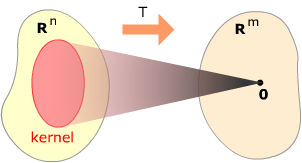
\includegraphics[width=0.5\textwidth]{img/kernel.png}
    \caption{Kernel Diagram}
\end{figure}

\defn{}{
    Let $T: V \to W$ be a linear transformation. The \textbf{range} of $T$, denoted by $\text{range}(T)$, is the set of all vectors in $W$ that are mapped to by $T$. 
    \[
        \text{range}(T) = \{T(\vec{v}) \in W : \vec{v} \in V\}
    \]
}
Note: If $T(\vec{v}) = A\vec{v}$, then $\text{range}(T) = \text{col}(A)$

\rmkb{
    Domain is the set of all possible inputs, codomain is the set of all possible outputs, and range is the set of all actual outputs.
}

\ex{
    $D^2 + D = 3I : C^{\infty} (\mathbb{R}) \to C^{\infty} (\mathbb{R})$ \\
    Find the kernel and range of $D^2 + D$.
    \[
        \ker(D^2 + D) = \{y \in C^{\infty} (\mathbb{R}) : (D^2 + D)(y) = 0\}
    \]
    \[
        = \{y \in C^{\infty} (\mathbb{R}) : y'' + y' = 0\}
    \]
}
Therefore, a homogenous linear differential equation is an example of a kernel.

\ex{
    Let $T:P_2 \to P_1$ be defined as follow:
    \[
        T(ax^2 + bx + c) = (a+b) + (b - c)x
    \] 
    Find the kernel and range of $T$. \\
    \textbf{Kernel:  } \\
    We want $(a+b) + (b - c)x = 0$ in $P_2$ \\
    Which is $0 + 0x$ in $P_1$ \\
    Therefore, $(a+b)$ and $(b-c)$ must be 0. \\
    \[
        \begin{bmatrix}
            \begin{array}{ccc|c}
                1 & 1 & 0 & 0 \\
                0 & 1 & -1 & 0
            \end{array}
        \end{bmatrix}
        =
        \begin{bmatrix}
            \begin{array}{ccc|c}
                1 & 0 & 1 & 0 \\
                0 & 1 & -1 & 0
            \end{array}
        \end{bmatrix}
    \]
    \[
        a = -c, b = c, c = c
    \]
    \[
        \ker(T) = \{-cx^2 + cx + c | c \in \mathbb{R}\}
    \]
    Write it as a spanned set: 
    \[
        \ker(T) = \text{span}\{-x^2 + x + 1\}
    \]
    \textbf{Range:}\\
    We want $(a+b) + (b - c)x$ in $P_1$ \\
    Let $b + ex $ be a generic element in $P_1$ \\
    Therefore, $d = a + b$ and $e = b - c$ \\
    We want to solve for $a, b, c$ in terms of $d, e$ \\
    \[
        \begin{bmatrix}
            \begin{array}{ccc|c}
                1 & 1 & 0 & d \\
                0 & 1 & -1 & e
            \end{array}
        \end{bmatrix}
        =
        \begin{bmatrix}
            \begin{array}{ccc|c}
                1 & 0 & 1 & d - e\\
                0 & 1 & -1 & e
            \end{array}
        \end{bmatrix}
    \]\\
    \[
        a = d - e -c, b = e + c, c \text{ is free}
    \]
    \[
        (a + b) + (b - c)x = (d - e + e + c) + (e + c - c)x = d + ex
    \]
    \[
        \text{range}(T) = \{d + ex | d, e \in \mathbb{R}\}
    \]
    So the range is all of $P_1(\mathbb{R})$.
}

\thmr{}{}{
    Let $T: V \to W$ be a linear transformation. Then:
    \begin{enumerate}
        \item $\ker(T)$ is a subspace of $V$
        \item $\text{range}(T)$ is a subspace of $W$
    \end{enumerate}
}

\pf{}

\ex{}

\thmr{Genearl Rank-Nullity Theorem}{Genearl Rank-Nullity Theorem}{
    Let $T: V \to W$ be a linear transformation. Then:
    \[
        \dim(V) = \dim(\ker(T)) + \dim(\text{range}(T))
    \]
}

\ex{}


\ex{}



\subsection{Linear transformation and basis}



\newpage

% % % ###############################################
\chapter{Eigenvalues and Eigenvectors}
\section{Lecture 19: }
\rmk{
    This lecture covers: 
    \begin{itemize}
        \item 6.1 Definition of Linear Transformations
        \item 6.2 Transformations of $\mathbb{R}^2$
        \item 6.3 The Kernel and Range of a Linear Transformation
    \end{itemize}
}















\newpage
\section{Lecture 20: Eigenspaces \& Eigenbase}
\rmk{
    This lecture covers: 
    \begin{itemize}
        \item 7.1 The Eigenvalue/Eigenvector Problem
        \item 7.2 General Results on Eigenvalues and Eigenvectors
        \item 7.3 Diagonalization
    \end{itemize}
}















\newpage


% % ###############################################
\chapter{Linear Differential Equations of Order n}
\section{Lecture 21: Linear Differential Equations}
\rmk{
    This lecture covers: 
    \begin{itemize}
        \item 8.1 General Theory of Linear Differential Equations
        \item 8.2 Constant Coefficient Homogeneous Linear Differential Equations
    \end{itemize}
}

\subsection{General Theory of Linear Differential Equations}
\defn{Linear Differential Equation}{
    A linear Differential Equation is an equation of the form
    \[
        y^{(n)} + \cdots + a_{n-1} (x) y' + a_n(x)y = F(x)
    \]
}

\defn{Homogeneous equation}{
    We have \textbf{Homogeneous equation} $F(x) = 0$ and \textbf{Non-homogeneous equation} $F(x) \neq 0$
}

\fact{
    The Differential operator $D$ is a linear Transformations
    \[
        D: C^1 (\mathbb{R}) \to C(\mathbb{R})
    \]
    given by $D(f) = y'$, and we extapolated to higher order derivatives. We define $L:C^n \mathbb{(R)} \to C(\mathbb{R})$:
    \[
        L = D^n + a_1(x)D^{n-1} + \cdots + a_{n-1}(x)D + a_n(x)I
    \]
    called the differential operator of order $n$. (the book leaves out the $I$ term)
}

\ex{
    % Consider y00 2y0 + exy = 0. Then a function y is a solution if and only if y satisfies Ly = 0, where L =.
    Consider $y'' + 2y' + e^x y = 0$. Then a function $y$ is a solution if and only if $y$ satisfies $Ly = 0$, where
    \[
        L =  D^2 + 2D + e^x I
    \]
    \[
        \text{Solution Set} = \{y | L(y) = 0\} = \ker(L)
    \]
    The solution set looks like this: \\
    If $y^{(n)} + a_{n-1}y^{(n-1)} + \cdots + a_1y' + a_0y = 0$  is a homogeneous linear differential equation of order $n$, then $y = c_1y_1 + \cdots + c_ny_n$ is a general solution, where $y_1, \cdots, y_n$ are linearly independent solutions.

}

\thmr{}{6.1.3}{
    \textbf{The set of solutions of a homogeneous linear differential equation of order $n$ is a vector space of dimension $n$}. It's the kernel of the linear map $L$. We call it the \textbf{solution space}.
}
% Any n linearly independent solutions y1 . . . , yn form a basis of the solution space. Every solution y can be expressed as a linear combination of basis vectors
% y = c1y1 + · · · + cnyn.
% The above expression is still called the general solution to the homogeneous equation.

Any $n$ linearly independent solutions $y_1, \cdots, y_n$ form a basis of the solution space. Every solution $y$ can be expressed as a linear combination of basis vectors
\[
    y = c_1y_1 + \cdots + c_ny_n
\]
The above expression is still called the general solution to the homogeneous equation.\\
\ex{
    Note that both $y_1 = \cos x$ and $y_2 = \sin x$ satisfy $y'' + y = 0$. Now we add information from linear algebra:
    \begin{itemize}
        \item We are talking about function spaces, so the vectors are functions (and the functions are vectors.)
        \item $\{\cos x, \sin x\}$ is independent. (How can we show this?) - Wronskian
        \item Any 2 independent functions in a 2-dimensional function space constitute a basis for the space.
        \item Any function in the space is a linear combination of basis vectors.
    \end{itemize}
    So we get the general solution, $y = c_1 \cos x + c_2 \sin x$. All solutions have this form.
}
\ex{
    Homogeneous, non-constant coefficients: Using trial solutions of the form $y = x^r$, find a basis for the solution space of
    \[
        2x^2y'' + 5xy' + y = 0
    \]
    on the interval $x > 0$ and the general solution.

    Trail solution: $y = x^r$ \\
    Goal: Figure out r \\
    Order: 2 \\
    Substitute $y = x^r$ into the equation:
    \[
        y' = rx^{r-1} \quad y'' = r(r-1)x^{r-2}
    \]
    \[
        2x^2r(r-1)x^{r-2} + 5xrx^{r-1} + x^r = 0
    \]
    \[
        2r(r-1)x^r + 5rx^r + x^r = 0
    \]
    \[
        x^r(2r^2 + 3r + 1) = 0
    \]
    \[
        (2r + 1)(r + 1) = 0
    \]
    \[
        r = -1/2, -1
    \]
    \[
        y_1 = x^{-1/2}, \quad y_2 = x^{-1}
    \]
    \[
        \boxed{y = c_1x^{-1/2} + c_2x^{-1}} \quad \text{General Solution}
    \]
    \rmkb{
        Note that this is a very specific case that shows when the sum of terms of $L$ is in the form of $c_ix^iD^i$.
    }
}


\subsection{Constant Coefficient Homogeneous Linear Differential Equations}

We build up a technique for solving order $n$ linear homogeneous diffeqs with constant coefficients.
\begin{enumerate}
    \item We start small by letting $L = D - aI$. Then $L(y) = y' - ay = 0$ has general solution $y = ce^{at}$.
    \item When $L$ has the form $L = (D - aI)(D - bI)$, the factors commute.
    \item If $y$ is a solution to $(D - a_iI)$, then
    \[
        (D - a_1I)(D - a_2I) \cdots (D - a_iI) \cdots (D - a_nI)y = 0,
    \]
    because the factors commute.
    \item Since the solution space is closed under addition and scalar multiplication, linear combinations of solutions to each factor are again solutions.
    \item We’ll call $p(r) = (r - a_1)(r - a_2) \cdots (r - a_n)$ the auxiliary polynomial.
\end{enumerate}



\subsubsection{Case 1: Distinct Real Roots}
\[
    p(r) = (r - a_1)(r - a_2) \cdots (r - a_n)
\]
\fact{
    $y_1 = e^{r_1x}, \ldots, y_n = e^{r_nx}$ are linearly independent solutions to $L(y) = 0$.
}

\thmr{More about Wronskian: }{}{

    Let $y_1, y_2, \ldots, y_n$ be solutions to the regular $n$-th order differential equation $Ly = 0$ on the interval $I$, and let $W$ denote their Wronskian. If $W(x_0) = 0$ at some point $x_0 \in I$, then $\{y_1, y_2, \ldots, y_n\}$ is linearly dependent on $I$. \\

    So, when the functions of interest are solutions to $Ly = 0$, \textbf{the Wronskian completely determines the independence of the functions}.

}

The general solution to the differential equation is
\[
    y = c_1e^{r_1x} + c_2e^{r_2x} + \cdots + c_ne^{r_nx}
\]
We use \textbf{initial conditions} to find the constants $c_1, c_2, \ldots, c_n$.

\ex{
    Solve the initial value problem: 
    \[
        y''-3y'-4y=0, \quad y(0)= 0 \quad y'(0) = 2
    \]
    \textbf{Step 1:} Find the general solution to the differential equation. \\
    We first write the Differential Equation in the form $L(y) = 0$:
    \[
        D^2 - 3D - 4I = 0
    \]
    \rmkb{
        Another way to think of this is to let $y = e^{rt}$.
    }
    The characteristic polynomial is
    \[
        P(r) = r^2 - 3r - 4 = (r - 4)(r + 1) = 0
    \]
    We set $P(r) = 0$ to find the root. The root is 
    \[
        r_1 = 4, \quad r_2 = -1
    \]
    each with multiplicity 1. So the general solution is
    \[
        y = c_1e^{4t} + c_2e^{-t}
    \]
    \textbf{Step 2:} Use the initial conditions to find the constants $c_1$ and $c_2$. \\
    We have $y(0) = 0$ and $y'(0) = 2$. We substitute these into the general solution:
    \[
        y(0) = c_1 + c_2 = 0
    \]
    \[
        y'(0) = 4c_1 - c_2 = 2
    \]
    We solve this system of equations to find $c_1$ and $c_2$.
    \[
        c_1 = \frac{2}{5}, \quad c_2 = -\frac{2}{5}
    \]
    \rmkb{
        For this step, we can also write the equation into matrix form and solve it using matrix algebra. e.g. 
        \[
            \begin{bmatrix}
                1 & 1 \\
                4 & -1
            \end{bmatrix}
            \begin{bmatrix}
                c_1 \\
                c_2
            \end{bmatrix}
            =
            \begin{bmatrix}
                0 \\
                2
            \end{bmatrix}
            =
            \begin{bmatrix}
                \begin{array}{cc|c}
                    1 & 0 & \frac{2}{5} \\
                    0 & 1 & -\frac{2}{5}
                \end{array}
            \end{bmatrix}
        \]
    }
    So the solution to the initial value problem is
    \[
        \boxed{ y = \frac{2}{5}e^{4t} - \frac{2}{5}e^{-t}}
    \]
}


\subsubsection{Case 2: Repeated Real Roots}
If $p(r)$ has repeated roots (some $r_i$ has multiplicity greater than 1), then solutions of the form $e^{rit}$ are not sufficient, as we will not get $n$ independent ones.

Note that $(D - aI)c_1te^{at} = c_1e^{at}$. So $(D - aI)^2(c_1te^{at} + c_2e^{at}) = 0$, and $\{e^{at}, te^{at}\}$ is an independent set.

Technique: If a real root $a$ appears with multiplicity $m$, then include the term
\[
    c_1e^{at} + c_2te^{at} + c_3t^2e^{at} + \cdots + c_mt^{m-1}e^{at}
\]
in the general solution.
\ex{
    Find the general solution to the diffeq
    \[
        y^{(4)} - 2y^{(3)} + y'' = 0.
    \]
    \textbf{Step 1:} Find the general solution to the differential equation. 
    \[
        P(r) = r^4 - 2r^3 + r^2 = r^2(r^2 - 2r + 1) = r^2(r-1)^2
    \]
    \[
        r_1 = 0 (m = 2), \quad r_2 = 1 (m = 2)
    \]
    The general solution is
    \[
        \boxed{y = c_1 + c_2t + c_3e^t + c_4te^t}
    \]
}



\subsubsection{Case 3: Complex Roots}
\defn{Euler's formula}{
    \[
        e^{i\theta} = \cos \theta + i\sin \theta
    \]
    In particular
    \[
        e^{ibt} = \cos(bt) + i\sin(bt) \text{, and } e^{-ibt} \text{ is the complex conjugate of } e^{ibt}
    \]
}

Suppose the (real) auxiliary polynomial $P(r)$ has complex roots $r = a \pm bi$. Then the complex conjugate $\overline{a+ib} = a - ib$ is also a root of $P(r)$.
\fact{
    The two complex valued functions $e^{(a \pm ib)t} = e^{at}e^{\pm ibt} = e^{at}(\cos(bt) \pm i \sin(bt))$ are two linearly independent solutions to the differential equation.

    These are complex-valued functions. We can obtain from them a pair of linearly independent, real functions. We set
    \[
        y_1 = \frac{e^{(a+ib)t} + e^{(a-ib)t}}{2} = e^{at}\cos(bt) \quad \text{and} \quad y_2 = \frac{e^{(a+ib)t} - e^{(a-ib)t}}{2i} = e^{at}\sin(bt).
    \]
    We conclude that the general real solution contains the term
    \[
        \boxed{c_1e^{at}\cos(bt) + c_2e^{at}\sin(bt)}
    \]
}

\ex{
    Solve the initial value problem $y'' - 6 y' + 25 y =0, y(0) = 0, y'(0) =1$
    \[
        P(r) = r^2 - 6r + 25 = (r-3)^2 + 16 = 0
    \]
    The roots are $r = 3 \pm 4i$. The general solution is
    \[
        y = c_1e^{3t}\cos(4t) + c_2e^{3t}\sin(4t)
    \]
    We substitute the initial conditions to find $c_1$ and $c_2$.
    \[
        y(0) = c_1 = 0
    \]
    \[
        y'(0) = 3c_1 + 4c_2 = 1
    \]
    \[
        c_2 = \frac{1}{4}
    \]
    So the solution to the initial value problem is
    \[
        \boxed{y = \frac{1}{4}e^{3t}\sin(4t)}
    \]

}

\subsubsection{Case 4: Repeated Complex Roots} (Analogous to repeated real roots–multiply by powers of $x$.) \\
Technique: If a (pair of) complex roots $a \pm ib$ appears with multiplicity $m$, then include
\[
    c_1e^{at}\cos(bt) + c_2e^{at}\sin(bt) + c_3te^{at}\cos(bt) + c_4te^{at}\sin(bt) + \cdots + c_{2m-1}t^{m-1}e^{at}\cos(bt) + c_{2m}t^{m-1}e^{at}\sin(bt)
\]
in the general solution.

\newpage
\ex{
    Find the general solution: $(D^2 + 4)^2(D + 1)y = 0$.
    \[
        P(r) = (r^2 + 4)^2(r + 1) = (r^2 + 4)(r^2 + 4)(r + 1)
    \]
    The roots are $r = 2i (m = 2), -2i (m = 2), -1 (m = 1)$. The general solution is
    \[
        y = c_1\cos(2t) + c_2\sin(2t) + c_3t\cos(2t) + c_4t\sin(2t) + c_5e^{-t}
    \]
}














\newpage
\section{Lecture 22: Annihilators}
\rmk{
    This lecture covers: 
    \begin{itemize}
        \item 8.3 The Method of Undetermined Coefficients: Annihilators
        \item 8.4 Complex-Valued Trial Solutions
    \end{itemize}
}















\newpage
\section{Lecture 23: Oscillations of a Mechanical System}
\rmk{
    This lecture covers: 
    \begin{itemize}
        \item 8.5 Oscillations of a Mechanical System
    \end{itemize}
}















\newpage

% % % % ###############################################
\chapter{Systems of Linear Differential Equations}
\section{Lecture 24: First Order Linear Systems}
\rmk{
    This lecture covers: 
    \begin{itemize}
        \item 9.1 First Order Linear Systems
        \item 9.2 Vector Formulation
        \item 9.3 General Results for First Order Linear Systems
    \end{itemize}
}

\rmkb{
    Today we are going to cover 9.1 to 9.3. We are going to skip many theorems. \\
    Next week we are going to do some examples for chapter 8. 
}

\subsection{Chapter 9.1: First Order Linear Systems}


\[
    \begin{bmatrix}
        x_1'(t) = a_{11}(t)x_1(t) + a_{12}(t)x_2(t) + \cdots + a_{1n}(t)x_n(t) + b_1(t) \\
        x_2'(t) = a_{21}(t)x_1(t) + a_{22}(t)x_2(t) + \cdots + a_{2n}(t)x_n(t) + b_2(t) \\
        \cdots \\
        x_n'(t) = a_{n1}(t)x_1(t) + a_{n2}(t)x_2(t) + \cdots + a_{nn}(t)x_n(t) + b_n(t) \\
    \end{bmatrix}
\]
The $b_i$ is the consists of the non-homogenous part.
If $b_i (t) = 0$, the system is homogenous. 



An example of the first-order linear system is:

\ex{
    \[
        x_1 ' = x_1 + 2x_2
    \]
    \[
        x_2 ' = 2x_1 + 2x_2
    \]
    \[
        x_1(0) = 1, x_2(0) = 0
    \]
}
The \textbf{Initial value} here is $x_1(0) = 1, x_2(0) = 0$.

A \textbf{solution} is an ordered n-tuple of functions $x_1(t), x_2(t), \dots, x_n(t)$ that satisfies the system of equations.

The solution will be in the form of: 
\ex{
    % \[
    %     x_1 ' = x_1 + 2x_2
    % \]
    % \[
    %     x_2 ' = 2x_1 + 2x_2
    % \]
    % \[
    %     x_1(0) = 1, x_2(0) = 0
    % \]
    \[
        x_1(t) = \text{Some function}, x_2(t) = \text{Some function}
    \]
}
Which is a vector of functions. 

There's a clever trick to solving the 2 by 2 system using the derivative, however, it is not that fast and no one use it in the exam so we are going to skip it. 


\rmkb{
    The first-order linear system is restrictive. However, we can transform a higher-order system by renaming functions.
}

\ex{
    \[
        \frac{d^2x}{dt^2} + 4e^t \frac{dx}{dt} - 9t^2x = 7t^2
    \]
    Strataegy: Let $x_1 = x$, $x_1' = x_2$
    \[
        x_1' = x_2
    \]
    \[
        x_2' = 9t^2x + 4e^t x_2 - 7t^2
    \]
    (Chapter 9.1)
}


\subsection{Chapter 9.2: Vector Formulation}
\rmkb{Chapter 9.2: How to transform the system into a matrix form.
}

\ex{
    Formulate with vectors. \\
    \[
        \vec{x}(t) = \begin{bmatrix}
            x_1(t) \\
            x_2(t) \\
            \cdots \\
            x_n(t)
        \end{bmatrix}
    \]
    \[
        \vec{x}'(t) = \begin{bmatrix}
            x_1'(t) \\
            x_2'(t) \\
            \cdots \\
            x_n'(t)
        \end{bmatrix}
    \]
    % \[
    %     A(t) = \begin{bmatrix}
    %         a_{11}(t) & a_{12}(t) & \cdots & a_{1n}(t) \\
    %         a_{21}(t) & a_{22}(t) & \cdots & a_{2n}(t) \\
    %         \cdots & \cdots & \cdots & \cdots \\
    %         a_{n1}(t) & a_{n2}(t) & \cdots & a_{nn}(t) 
    %     \end{bmatrix}

    % \]
    \[
        A(t) = \begin{bmatrix}
            a_{11}(t) & a_{12}(t) & \cdots & a_{1n}(t) \\
            a_{21}(t) & a_{22}(t) & \cdots & a_{2n}(t) \\
            \cdots & \cdots & \cdots & \cdots \\
            a_{n1}(t) & a_{n2}(t) & \cdots & a_{nn}(t)
        \end{bmatrix}
    \]
    Coefficient matrix: \\
    \[
        \vec{b}(t) = \begin{bmatrix}
            b_1(t) \\
            b_2(t) \\
            \cdots \\
            b_n(t)
        \end{bmatrix}
    \]

}   

\thmr{}{}{
    $V_n(I)$ is a column vector of $n$ functions defined on an interval $I$.
}

\newpage

\ex{
    \[
        \begin{bmatrix}
            e^{3t} \\
            2\\
            e^{7t}
        \end{bmatrix}
        \in V_3(\mathbb{R})
    \]
    for any fixed $n$, $I$, $V_n(I)$ is a vector space.
}




\subsubsection{Wronskian}
\rmkb{
    We do not test this
}
Wronskan of a set of $n$ column vectors in $V_n(I)$ 

Wronskien of $\{\vec{x}_1, \vec{x}_2, \cdots, \vec{x}_n \}$

$W(t) = \text{Wronskian} = \begin{bmatrix}
    \vec{x}_1 & \vec{x}_2 & \cdots & \vec{x}_n
\end{bmatrix}  $

\thmr{}{}{
    If $W(t) \neq 0$ for all $t \in I$, then $\{\vec{x}_1, \vec{x}_2, \cdots, \vec{x}_n \}$ is linearly independent. 
}

\thmr{}{}{
    If $\{\vec{x}_1, \vec{x}_2, \cdots, \vec{x}_n \}$ is linearly independent, then $W(t) \neq 0$ for all $t \in I$. 
}


\subsection{Chapter 9.3: Genearl results for first-order linear systems}
\thmr{Initial value problem}{}{
    $\vec{x}'(t) = A(t) \vec{x}(t) + \vec{b}(t)   $ and $\vec{x}(t_0) = \vec{x}_0$ has a unique solution on an interval $I$ containing $t_0$ if $A(t)$ and $\vec{b}(t)$ are continuous on $I$.
}   



\thmr{9.3.2}{}{
    The set of solutions to the homogenous system $\vec{x}'(t) = A(t) \vec{x}(t)$ is a vector space of dimension $n$.
}

\subsubsection{Fundamental solution set}
The fundamental solution set is basically a basis for the solution space.

\thmr{The fundamental solution set}{}{
    \[
        S = \{
            x_1, x_2, \cdots, x_n
        \}
    \]
    S is a set of solutions to the homogenous system $\vec{x}'(t) = A(t) \vec{x}(t)$ that are linearly independent.
}

The non-homogenous case:
\[
    \vec{x} = c_1 \vec{x}_1 + c_2 \vec{x}_2 + \cdots + c_n \vec{x}_n + \boxed{\vec{x}_p}
\]

We add a single solution to the homogenous system to the solution of the non-homogenous system.


Simplifying assumptions:
\[
    \vec{x}'(t) = A\vec{x}(t)
\]
is homogenous and $A$ is a matrix of constants and $A$ is non-defective.

\rmkb{
    Recall: Non-defective means that the matrix has $n$ linearly independent eigenvectors.
}

\thmr{}{}{
    Let $A$ be a $n \times n$ matrix of real constants, and let $\lambda$ be a real eigenvalue of corresponding to the eigenvector $\vec{v}$. \\
    
    Then 
    \[
        \vec{x}(t) = e^{\lambda t} \vec{v}
    \]
    is a solution to the homogenous system $\vec{x}'(t) = A\vec{x}(t)$.
}
\rmkb{
    Recall: Means that $A\vec{v} = \lambda \vec{v}$
}

\pf{
    If $\vec{x}(t) = e^{\lambda t} \vec{v}$, then
    \[
        A(e^{\lambda t} \vec{v}) = e^{\lambda t} A\vec{v} = e^{\lambda t} \lambda \vec{v} = \lambda e^{\lambda t} \vec{v}
    \]
    On the other side, if I take the derivative of $\vec{x}(t)$, I get
    \[
        \vec{x}'(t) = \lambda e^{\lambda t} \vec{v}
    \]
    We notice that the two sides are equal.
}

And we are going to have enough solutions to form a basis for the solution space.


\thmr{}{}{
    If $A$ has $n$ real eigenvectors $\vec{v}_1, \vec{v}_2, \cdots, \vec{v}_n$ with corresponding real eigenvalues $\lambda_1, \lambda_2, \cdots, \lambda_n$, then 
    \[
        \vec{x}_k = e^{\lambda_k t} \vec{v}_k
    \]
    is a solution to the homogenous system $\vec{x}'(t) = A\vec{x}(t)$.

}
\newpage

\ex{
    \[
        A = \begin{bmatrix}
            1 & 2 \\
            2 & -2
        \end{bmatrix}
    \]
    The eigenvalue is: \\
    \[
        | A - \lambda I | = (1 - \lambda) \cdot (-2 - \lambda) - 4 = 0
    \]
    \[
        \lambda = 2, -3
    \]
    nullspace of $A - 2I$ is $\begin{bmatrix}
        -1 & 2 \\
        2 & -4
    \end{bmatrix} \to \begin{bmatrix}
        1 & -2 \\
        0 & 0
    \end{bmatrix} 
    $ \[
        \vec{v}_1 = \begin{bmatrix}
            2 \\
            1
        \end{bmatrix}
    \]
    nullspace of $A + 3I$ is $\begin{bmatrix}
        4 & 2 \\
        2 & 1
    \end{bmatrix} \to \begin{bmatrix}
        2 & 1 \\
        0 & 0
    \end{bmatrix}
    $ \[
        \vec{v}_2 = \begin{bmatrix}
            -1 \\
            2
        \end{bmatrix}
    \]
    \textbf{What's new today:} \\
    Solution = \\
    \[
        \begin{bmatrix}
            x_1 \\ x_2
        \end{bmatrix}
        =
        c_1 e^{2t} \begin{bmatrix}
            2 \\ 1
        \end{bmatrix}
        +
        c_2 e^{-3t} \begin{bmatrix}
            -1 \\ 2
        \end{bmatrix}
    \]
    \[
        x_1 = 2 c_1 e^{2t} - c_2 e^{-3t}
    \]
    \[
        x_2 = c_1 e^{2t} + 2c_2 e^{-3t}
    \]

    Initial values: \\
    \[
        x_1(0) = 2c_1 - c_2 = 1
    \]
    \[
        x_2(0) = c_1 + 2c_2 = 0
    \]
    \[
        \begin{bmatrix}
            \begin{array}{cc|c}
                2 & -1 & 1 \\
                1 & 2 & 0
            \end{array}
        \end{bmatrix}
        \to
        \begin{bmatrix}
            \begin{array}{cc|c}
                1 & 2 & 0 \\
                2 & -1 & 1
            \end{array}
        \end{bmatrix}
        \to
        \begin{bmatrix}
            \begin{array}{cc|c}
                1 & 2 & 0 \\
                0 & -5 & 1
            \end{array}
        \end{bmatrix}
        \to
        \begin{bmatrix}
            \begin{array}{cc|c}
                1 & 0 & 2/5 \\
                0 & 1 & -1/5
            \end{array}
        \end{bmatrix}
    \]

}


\ex{
    \[
        \vec{x' = A\vec{x}}
    \]
    \[
        A = \begin{bmatrix}
            0 & 4 \\
            1 & 0
        \end{bmatrix}
    \]
    \[
        x_1' = 4x_2
    \]
    \[
        x_2' = x_1
    \]
    \textbf{Step 1: Find the eigenvalues and eigenvectors} \\
    \[
        |A - \lambda I| = \begin{bmatrix}
            -\lambda & 4 \\
            1 & -\lambda
        \end{bmatrix} = \lambda^2 - 4 = 0
    \]
    \[
        \lambda _1 = 2, \lambda_2 = -2
    \]
    \textbf{For $\lambda_1 = 2$} \\
    \[
        \begin{bmatrix}
            -2 & 4 \\
            1 & -2
        \end{bmatrix} \to \begin{bmatrix}
            1 & -2 \\
            0 & 0
        \end{bmatrix}
    \]
    \[
        \boxed{\vec{v}_1 = \begin{bmatrix}
            2 \\
            1
        \end{bmatrix}}
    \]
    \textbf{For $\lambda_2 = -2$} \\
    \[
        \begin{bmatrix}
            2 & 4 \\
            1 & 2
        \end{bmatrix} \to \begin{bmatrix}
            1 & 2 \\
            0 & 0
        \end{bmatrix}
    \]
    \[
        \boxed{\vec{v}_2 = \begin{bmatrix}
            -2 \\
            1
        \end{bmatrix}}
    \]
    \textbf{Step 2: Write the general solution} \\
    \[
        \begin{bmatrix}
            x_1 \\ x_2
        \end{bmatrix}
        =
        c_1 e^{2t} \begin{bmatrix}
            2 \\ 1
        \end{bmatrix}
        +
        c_2 e^{-2t} \begin{bmatrix}
            -2 \\ 1
        \end{bmatrix}
    \]
}

\rmkb{
    If you can not zero out the second role, it means that you are wrong. 
}


Let's do a 3 by 3 example.
We will leave the complex case for the next lecture.s

\ex{
    \[
        A = \begin{bmatrix}
            0 & -3 & 1 \\
            -2 & -1 & 1 \\
            0 & 0& 2
        \end{bmatrix}
    \]
    \textbf{Step 1: Find the eigenvalues and eigenvectors} \\
    \[
        |A - \lambda I| = 
        \begin{bmatrix}
            0 - \lambda & -3 & 1 \\
            -2 & -1 - \lambda & 1 \\
            0 & 0 & 2 - \lambda
        \end{bmatrix}
        = 0
    \]
    Characteristic polynomial: \\
    \[
        (2 - \lambda)(\lambda -3) (\lambda - 2) = 0
    \]
    \[
        \lambda_1 = 2, \lambda_2 = -3, \lambda_3 = 2
    \]
    \textbf{For $\lambda_1 = 2$} \\
    \[
        \begin{bmatrix}
            -2 & -3 & 1 \\
            -2 & -3 & 1 \\
            0 & 0 & 0
        \end{bmatrix} \to \begin{bmatrix}
            -2 & -3 & 1 \\
            0 & 0 & 0 \\
            0 & 0 & 0
        \end{bmatrix}
    \]
        $x_2, x_3 $ are free
    \[
        -2x_1 = 3x_2 - x_3
    \]
    \[
        x_1 = -\frac{3}{2} x_2 + \frac{1}{2} x_3
    \]

    \[
        \vec{v}_1 = (3, -2, 0)
    \]
    \[
        \vec{v}_2 = (1, 0, 2)
    \]

    \textbf{For $\lambda_2 = -3$} \\
    \[
        \begin{bmatrix}
            3 & -3 & 1 \\
            -2 & 2 & 1 \\
            0 & 0 & 5
        \end{bmatrix} \to \begin{bmatrix}
            1 & -1 & 0 \\
            0 & 0 & 1\\
            0 & 0 & 0
        \end{bmatrix}
    \]
    $x_2$ is free
    \[
        x_1 = x_2
    \]
    \[
        x_3 = 0
    \]
    \[
        \vec{v}_3 = (1, 1, 0)
    \]

    \textbf{Step 2: Write the general solution} \\
    \[
        \begin{bmatrix}
            x_1 \\ x_2 \\ x_3
        \end{bmatrix}
        =
        c_1 e^{2t} \begin{bmatrix}
            3 \\ -2 \\ 0
        \end{bmatrix}
        +
        c_2 e^{-3t} \begin{bmatrix}
            1 \\ 0 \\ 2
        \end{bmatrix}
        +
        c_3 e^{2t} \begin{bmatrix}
            1 \\ 1 \\ 0
        \end{bmatrix}
    \]

}









\newpage
\section{Lecture 25: }
\rmk{
    This lecture covers: 
    \begin{itemize}
        \item 
    \end{itemize}
}
\subsection{Complex-Valued Solutions}
\thmr{}{}{
    Let $\vec{u}(t)$ and $\vec{v}(t)$ be real-valued vector functions. If \\
    \[
        \vec{w}_1(t) = \vec{u}(t) + \vec{v}(t) \quad \text{and} \quad \vec{w}_2(t) = \vec{u}(t) - \vec{v}(t)
    \]
    are complex conjugate solutions to $x' = Ax$ , then\\
    \[
        x_1(t) = \vec{u}(t) \text{and} \quad x_2(t) = \vec{v}(t)
    \]
    are themselves real-valued solutions to $x' = Ax$.
}

\ex{
    Let $A = \begin{bmatrix} 0 & 2 \\ -2 & 0 \end{bmatrix}$. Find the general solution to $x' = Ax$. \\ \\
    \textbf{Step 1: Find the Eigenvalues and Eigenvectors} \\
    The characteristic equation is $\lambda^2 + 4 = 0$, so $\boxed{\lambda = \pm 2i}$. 

    For $\lambda = 2i$, we have
    \[
        \begin{bmatrix} -2i & 2 \\ -2 & -2i \end{bmatrix} \begin{bmatrix} x_1 \\ x_2 \end{bmatrix} = \begin{bmatrix} 0 \\ 0 \end{bmatrix}
    \]
    RREF: \\
    \[
        \begin{bmatrix} 
            \begin{array}{cc|c}
                1 & i & 0\\ 0 & 0 &0
            \end{array}
        
        \end{bmatrix}
    \]

    So, $\boxed{\vec{v}_1 = \begin{bmatrix} -i \\ 1 \end{bmatrix}}$ or $\boxed{\vec{v}_2 = \begin{bmatrix} 1 \\ i \end{bmatrix}}$ is an eigenvector corresponding to $\lambda = \pm 2i$. \\

    \textbf{Step 2: Find the General Solution} \\
    The general solution is
    \[
        x(t) = c_1e^{2it}\begin{bmatrix} -i \\ 1 \end{bmatrix} + c_2e^{-2it}\begin{bmatrix} 1 \\ i \end{bmatrix}
    \]
    \[
        = c_1\begin{bmatrix} -i\cos(2t) - \sin(2t) \\ \cos(2t) - i\sin(2t) \end{bmatrix} + c_2\begin{bmatrix} \cos(2t) - i\sin(2t) \\ i\cos(2t) - \sin(2t) \end{bmatrix}
    \]
    Here, we want it to be in the form of $\vec{u}(t) + i \vec{v}(t)$. So, we can rewrite the general solution as \\
    \[
        = \begin{bmatrix} c_1\cos(2t) + c_2\sin(2t) \\ c_2\cos(2t) - c_1\sin(2t) \end{bmatrix} + i\begin{bmatrix} c_2\cos(2t) - c_1\sin(2t) \\ c_1\cos(2t) + c_2\sin(2t) \end{bmatrix}
    \]
    
    \[
        = \begin{bmatrix} c_1\cos(2t) + c_2\sin(2t) \\ c_2\cos(2t) - c_1\sin(2t) \end{bmatrix} + i\begin{bmatrix} c_2\cos(2t) - c_1\sin(2t) \\ c_1\cos(2t) + c_2\sin(2t) \end{bmatrix}
    \]



    
}








\newpage

\ex{
    \textbf{Example 1:} $(D^2 + 2D +10)^2$
    The first step is to find the order of this, which is 2 inside from $D^2$ and squared it to get $\boxed{4}$. \\

    \[
        p(r) = r^2 + 2r + 10 = 0
    \]
    Which doesn't obviously factor, so we check: \\
    \[
        b^2 - 4ac = 4 - 40 = \boxed{-36}
    \]
    Which is negative, so we have complex roots. \\
    \[
        r = \frac{-b \pm \sqrt{b^2 - 4ac}}{2a} = \frac{-2 \pm \sqrt{-36}}{2} = \frac{-2 \pm 6i}{2} =\boxed{ -1 \pm 3i}
    \]

    The multiplicity of the roots is 2 for each, so we have to use the formula: \\
    \[
        e^{rt} = e^{-t}(\cos(3t) \pm i\sin(3t))
    \]

    The general solution is: \\
    \[
        \boxed{        
            y = c_1 e^{-t}\cos(3t) + c_2 e^{-t}(\sin(3t)) + c_3 te^{-t}(\cos(3t)) + c_4 te^{-t}(\sin(3t))
        }    
    \]
}

\ex{
    \textbf{Example 2:} $y''' - y'' +y' -y = 0$ \\
    \[
        p(r) = r^3 - r^2 + r - 1 = 0
    \]
    \[
        = r^2 (r - 1) + 1(r - 1) 
    \]
    \[
        = (r +1) (r - 1)^2 = 0
    \]

    Rational root Theorem: \\
    Trial:
    \[
        r = \pm 1
    \]
    try $r = 1$:
    \[
        1 - 1 + 1 - 1 = 0
    \]
    So, we have a root of 1. \\
    \[
       \boxed{ y = c_1e^t + c_2 \cos(t) + c_3 \sin(t)}
    \]

}


\newpage
\ex{
    \textbf{Example 3:} $y'' + y = 6xe^x$ \\
    $y_c$ = \text{General solution to }$y'' + y = 0$ \\
    $y_p = \text{Trial solution} $ \\
    $y_c$:  
    \[
        p(r) = r^2 + 1 = 0
    \] 
    \[
        r = \pm i
    \]
    \[
        y_c = c_1\cos(x) + c_2\sin(x)
    \]
    \[
        y(p) = Ae^x + Bxe^x
    \]
    Apply $(D^2 + I) y_p$ \\
    \[
        D(Ae^x + Bxe^x) 
    \]
    \[
        = Ae^x + Be^x + Bxe^x
    \]
    \[
        = (A + B)e^x + Bxe^x
    \]
    \[
        D^2(Ae^x + Bxe^x) = (A + B)e^x + Be^x + Bxe^x
    \]
    \[
        = (A + B)e^x + 2Be^x + Bxe^x
    \]
    \[
        y = c_1 e^t + c_2 \cos(t) + c_3 \sin(t) 
    \]
    \[
        (D^2+I) y_p = (A + 2B) e^x + Bxe^x + Ae^x + Bxe^x
    \]
    \[
        = (2A + 2B)e^x + 2Bxe^x
    \]
    \[
        = 6xe^x
    \]
    \[
        2A + 2B = 0
    \]
    \[
        2B = 6
    \]
    \[
        B = 3
    \]
    \[
        A = -3
    \]
    \[
        y = c_1 
    \]



}









\newpage


\chapter{Review}
\section{S15 FQ6}
% Let M2×2(R) be the vector space of 2×2 real matrices. Consider the linear
% transformation T : M2×2(R) → M2×2(R) defined by
% "a b#! "a+d b−c#
% T cd =a−cb+d.

Let $M_{2 \times 2}(\mathbb{R})$ be the vector space of $2 \times 2$ real matrices. Consider the linear transformation $T : M_{2 \times 2}(\mathbb{R}) \to M_{2 \times 2}(\mathbb{R})$ defined by
\[
    T \begin{pmatrix}
        \begin{bmatrix}
            a & b \\
            c & d
        \end{bmatrix}
    \end{pmatrix}
     = \begin{bmatrix}
        a + d & b - c \\
        a - c & b + d
    \end{bmatrix}.
\]

\textbf{Kernel:} 

\[
    a+d = 0 \quad b-c = 0 \quad a-c = 0 \quad b+d = 0
\]
\[
    a = c = b = -d
\]

Therefore, the basis for the kernel is: 
\[
    \begin{bmatrix}
        1 & 1 \\
        1 & -1
    \end{bmatrix}
\]

So the nullity of $T$ is 1.


\textbf{Range: }

\[
    \begin{bmatrix}
        a + d & b - c \\
        a - c & b + d
    \end{bmatrix}
    = a \begin{bmatrix}
        1 & 0 \\
        1 & 0
    \end{bmatrix}
    + b \begin{bmatrix}
        0 & 1 \\
        0 & 1
    \end{bmatrix}
    + c \begin{bmatrix}
        0 & -1 \\
        -1 & 0
    \end{bmatrix}
    + d \begin{bmatrix}
        1 & 0 \\
        0 & 1
    \end{bmatrix}
\]

However, these for vectors are not linearly independent: \\
\[
    \begin{bmatrix}
        1 & 0 \\
        0 & 1
    \end{bmatrix}
    =
    \begin{bmatrix}
        1 & 0 \\
        1 & 0
    \end{bmatrix}
    +
    \begin{bmatrix}
        0 & 1 \\
        0 & 1
    \end{bmatrix}
    +
    \begin{bmatrix}
        0 & -1 \\
        -1 & 0
    \end{bmatrix}
\]

Therefore, the basis for the range is:
\[
    \begin{bmatrix}
        1 & 0 \\
        1 & 0
    \end{bmatrix}
    \quad
    \begin{bmatrix}
        0 & 1 \\
        0 & 1
    \end{bmatrix}
    \quad
    \begin{bmatrix}
        0 & -1 \\
        -1 & 0
    \end{bmatrix}
\]
and the rank of $T$ is 3.\\
\textbf{Conclusion:}
This aligned with the Rank-Nullity Theorem, as the rank of $T$ is 3 the nullity is 1, and the sum of the rank and nullity is 4, which is the dimension of the domain of $T$.

\end{document}
